\section{Background}
The reduced-complexity approach to delta modeling employed in \textit{pyDeltaRCM} hinges upon the notion of the random walk \cite{Pearson1905}.
To approximate physics, the DeltaRCM methodology does not use a truly random walk and rather weights the transport pathways of water and sediment to approximate physical processes.
As a result, an individual model run represents a single stochastic realization for a given parameter set. 
The variability in the model run behavior is also expected to result in runtime variability.
Understanding the variability in run times for any given set of model parameters can help estimate the required computational time to conduct a set of numerical experiments and can also be used to set wall-clock times for model runs conducted on HPC clusters. 

\section{Model Runs}
A set of 100 small model runs are conducted to develop an understanding of the variability in model run time for a fixed set of parameters.
The following YAML file is used to conduct the model runs.
For these realizations a special subclass of the standard \textit{pyDeltaRCM} model is used which tracks and records the number of sediment parcel iterations conducted in each realization.
The underlying hypothesis is that the sediment parcel iteration process consumes the majority of the model runtime, and therefore one would expect to see a correlation between the number of sediment parcel iterations and the runtime for any given realization.\\

\noindent \texttt{YAML} configuration file: \vspace{-6pt}
\begin{boxedverbatim}
timesteps: 1500
ensemble: 100
Length: 4000.0
Width: 7000.0
dx: 50.0
L0_meters: 50.0
u0: 1.0
N0_meters: 250.0
h0: 5.0
save_dt: 250000
save_metadata: True
save_eta_grids: True
SLR: 48e-10  # small background SLR
f_bedload: 0.5
\end{boxedverbatim}

\section{Results}
The 100 runs completed with an average runtime of 2.025 hours per run, and a standard deviation of 0.082 hours. 
A histogram of the runtimes for the 100 runs with a kernel-density estimated smoothed PDF overlaid is provided (Figure \ref{fig:runtimes}, second row).
These results reveal a disparity of about 0.5 hours between the slowest and the fastest realization, significant ($\sim25\%$) in the context of runs that are taking an average of just 2 hours to complete. 

\begin{figure}[!ht]
	\makebox[\textwidth][c]{
	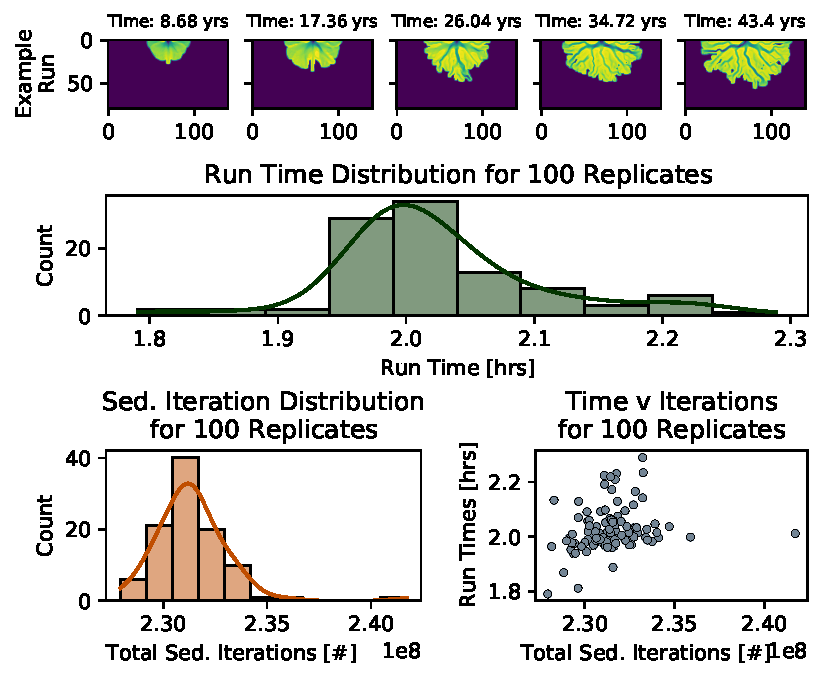
\includegraphics[width=\textwidth]{RuntimeVariability/figs/runtimes.pdf}
	}	
	\caption{Results from the 100 runs generated by the YAML configuration file. \textit{Top row:} Evolution of model topography from a single realization. \textit{Second row:} Run time distribution for the 100 runs, histogram shown with Kernel Density Estimated PDF. \textit{Bottom Left:} Distribution of the total sediment parcel iterations for the 100 runs. \textit{Bottom Right:} Cross-plot of the 100 model run times against the total sediment parcel iterations.}
	\label{fig:runtimes}
\end{figure}

\section{Conclusions}
There appears to be a non-negligible degree of variability in the run times for different realizations run from the same parameter set.
This variability is not directly linked to the number of sediment parcel iterations, as a strong correlation between run time and total sediment parcel iterations does not exist (Figure \ref{fig:runtimes}, bottom right).
When planning a set of numerical experiments, if one or two prototype runs have been conducted to test the parameter set and the size of the domain, the computational time required to conduct a larger ensemble of runs can be estimated conservatively by inflating the prototype run times by $\sim25\%$ and multiplying that value by the number of simulations being run.

\clearpage
\bibliographystyle{plainnat}
\bibliography{bib/bib}